%%%%%%%%%%%%%%%%

% designed to be integrated with conceptual figure

%%%%%%%%%%%
\documentclass[border=0.2cm,11pt]{standalone}
\usepackage{tgheros}
\renewcommand*\familydefault{\sfdefault}%

\usepackage{tikz}
\usetikzlibrary{positioning,automata}
\usetikzlibrary{shapes}

\tikzset{>=latex} % for LaTeX arrow head
\usepackage{xcolor}

% taken from neural networks
\usepackage{amsmath} % for aligned
%\usepackage{amssymb} % for \mathbb
%\usepackage{etoolbox} % for \ifthen
\usepackage{listofitems} % for \readlist to create arrays
\usetikzlibrary{arrows.meta} % for arrow size
\usepackage[outline]{contour} % glow around text
\contourlength{1.4pt}

% using tableau 10 color palette: https://public.tableau.com/views/TableauColors/ColorPaletteswithRGBValues?%3Aembed=y&%3AshowVizHome=no&%3Adisplay_count=y&%3Adisplay_static_image=y

\definecolor{myblue}{RGB}{31,119,180}
\definecolor{myred}{RGB}{214,39,40}
\definecolor{mygreen}{RGB}{44,160,44}

% original colors defined by original author
\colorlet{myorange}{orange!70!red!60!black}
\colorlet{mydarkred}{red!30!black}
\colorlet{mydarkblue}{blue!40!black}
\colorlet{mydarkgreen}{green!30!black}
\tikzstyle{mynode}=[align=center, rounded corners, minimum height=1cm]
\tikzstyle{procs_ecolo}=[mynode, rectangle, fill=mygreen!30]
\tikzstyle{procs_evol}=[mynode, rectangle, fill=myred!30]
\tikzstyle{mechanisms}=[mynode, rectangle, thick, minimum width=3cm]
\tikzstyle{patterns}=[mynode, circle, thick, fill=myblue!20]


% \tikzstyle{node}=[ultra thick,circle,minimum size=30,inner sep=2.,outer sep=0.6]
% \tikzstyle{node green}=[node,fill=mygreen]
% \tikzstyle{node blue}=[node,fill=myblue]
% \tikzstyle{node orange}=[node,orange!20!black,draw=myorange!30!black,fill=myorange!20]
% \tikzstyle{node red}=[node,fill=myred]
\tikzstyle{connect}=[thick,mydarkblue] %,line cap=round
\tikzstyle{connect arrow}=[-{Latex[length=6,width=6]},thick,mydarkblue,shorten <=0.5,shorten >=1]
 

% spacing nodes
% \tikzset{node distance = 0.5cm and 0.5cm}

\begin{document}

 
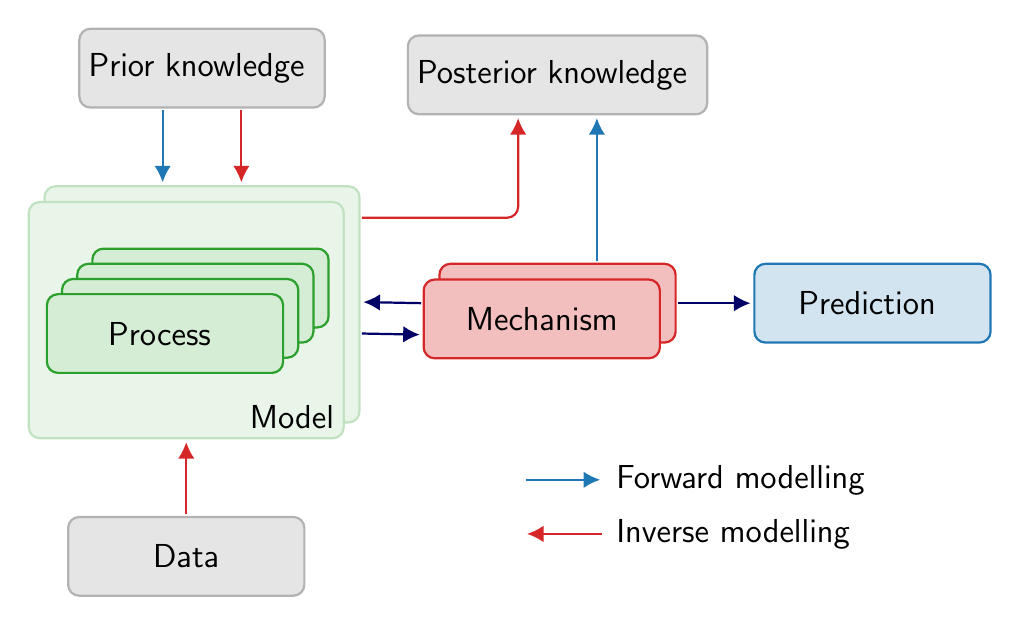
\begin{tikzpicture}[
    node distance=4cm,
    on grid,
    very thick,
    font=\large]
 
\node[mechanisms, draw=mygreen!30, minimum height = 3.cm, minimum width = 4cm,fill=mygreen!10] (model_contour) at (-2.5,-2.5) {};
\node[mechanisms, draw=mygreen!30, minimum height = 3.cm, minimum width = 4cm,fill=mygreen!10] (model_contour2) at ([xshift=-0.2cm,yshift=-0.2cm]model_contour.center) {};

\node[above left] at (model_contour2.south east) {Model};


\foreach \Z in {1,...,4}{
    \node[mechanisms, fill=mygreen!20,draw=mygreen] at (-2.2,-2.1,\Z/2) (procs\Z) { Process };
}

\node[mechanisms, fill=myred!30,draw=myred] (mechs2) [right=4.6cm of procs2] {  };
\node[mechanisms, fill=myred!30,draw=myred] (mechs) at ([xshift=-0.2cm,yshift=-0.2cm]mechs2.center) {Mechanism};

% \node[mechanisms, fill=mygreen!30, below left =of mechs] (struc) { Structure };

\node[mechanisms, fill=myblue!20,draw=myblue] (patt) [right= of mechs2]{ Prediction };

\node[mechanisms,draw=black!30,fill=black!10,] (data) [below= 3cm of model_contour2]{ Data};
\node[mechanisms,draw=black!30,fill=black!10,] (prior_knowledge) [above= 3cm of model_contour]{ Prior knowledge };
\node[mechanisms,draw=black!30,fill=black!10,] (post_knowledge) [above= 2.9cm of mechs2]{ Posterior knowledge };

\begin{scope} [connect arrow]  % now dashed is for the lines inside the scope
    % \draw (procs1) to [bend right] (model_contour.east)  ; 
    % \draw (patt.north) to [bend right] (mechs)  ; 

    % \draw (patt.north) to [bend right] (model_contour.east)  ; 
    \draw ([yshift=-0.37cm]model_contour.east) to ([yshift=-0.2cm]mechs.west); 
    \draw ([yshift=0.2cm]mechs.west) to ([yshift=0.03cm]model_contour.east);

    \draw (mechs2.east) to (patt.west); 


    \draw[myred] (data) to  (model_contour2.south)  ; 
    % \draw[myred] ([xshift=0.5cm]model_contour.north) to  ([xshift=0.5cm]prior_knowledge.south)  ; 
    \draw[myblue] ([xshift=-0.5cm]prior_knowledge.south) to  ([xshift=-0.5cm]model_contour.north)  ; 
    \draw[myred] ([xshift=0.5cm]prior_knowledge.south) to  ([xshift=0.5cm]model_contour.north)  ; 
    \draw[myred,rounded corners] ([yshift=1.1cm]model_contour.east) -| ([xshift=-0.5cm]post_knowledge.south); 

    \draw[myblue] ([xshift=0.5cm]mechs2.north) to ([xshift=0.5cm]post_knowledge.south); 
    % \draw[myred] ([xshift=0.5cm]mechs2.north)to ([xshift=0.5cm]post_knowledge.south); 

    \path ([xshift=0cm,yshift=2cm]current bounding box.south)
    node[matrix,anchor=north west,cells={nodes={anchor=west}},thick,inner sep=1ex]{
     \draw[myblue](0,0) -- ++ (1,0); & \node[black]{Forward modelling};\\
     \draw[myred](1,0) -- ++ (-1,0); & \node[black]{Inverse modelling};\\
    };

\end{scope}

\end{tikzpicture}
 
\end{document}